% Τεκμηρίωση δεύτερης ερευνητικής εργασίας του μαθήματος ΓΡΑΦΙΚΗ ΥΠΟΛΟΓΙΣΤΩΝ

\documentclass[12pt]{report}
\usepackage[a4paper, margin=3cm, bottom=3cm]{geometry} 
\linespread{1.3} % διάστιχο: 1,5
\usepackage{tempora} % κάνει την γραμματοσειρά Times New Roman
\usepackage[LGR, T1]{fontenc}
\usepackage[utf8]{inputenc}
\usepackage[greek]{babel}
\usepackage{hyperref}
\usepackage[pdftex]{graphicx}
\graphicspath{{images/}}
\usepackage{alphabeta}
\usepackage{gensymb}
\usepackage{amsmath}
\usepackage{chngcntr}
\usepackage{attachfile2}

% μικρότερη γραμματοσειρά τίτλων κεφαλαίων και προεπιλεγμένη απόσταση κεφαλαίων και ενοτήτων
\usepackage{titlesec}
\titleformat{\chapter}[hang]{\Huge\bfseries}{\thechapter{. }}{0pt}{\Huge\bfseries}
\titlespacing*{\chapter} {0pt}{10pt}{20pt}
\titlespacing*{\section} {0pt}{3.5ex plus 1ex minus .2ex}{2.3ex plus .2ex}

\usepackage[labelfont=bf]{caption}
\addto\captionsgreek{\renewcommand{\figurename}{Εικόνα}}
\usepackage[bottom]{footmisc}

% δεν δημιουργεί καινούργια σελίδα στην αρχή κάθε κεφαλαίου
\usepackage{etoolbox}
\makeatletter
    \patchcmd{\chapter}{\if@openright\cleardoublepage\else\clearpage\fi}{}{}{}
\makeatother

\begin{document}
\renewcommand\bibname{Αναφορές}

\pagenumbering{arabic}

% Πρώτη σελίδα: Επιγραφή

\begin{titlepage}

\begin{center}


\includegraphics[width=0.5\textwidth]{images/uthlogo}\\
\vspace{3em}

\Large \textbf {Προβολές \textlatin{Cavalier} και \textlatin{Cabinet} - Μοναδιαίος κύβος}\\
\vspace{1.5em}
\normalsize από τις \\
\vspace{1.5em}
\textup{\small {\bf Όλγα Βασιλείου} [\textlatin{\href{mailto:vaolga@uth.gr}{vaolga@uth.gr}}]\\ \vspace{.5em} {\bf Βαΐα Γιαννάδη} [\textlatin{\href{mailto:gvaia@uth.gr}{gvaia@uth.gr}}]}

\vspace{4in}
Τμήμα Πληροφορικής με Εφαρμογές στη Βιοϊατρική \\
Σχολή Θετικών Επιστημών, Πανεπιστήμιο Θεσσαλίας, Λαμία
\vspace{2em}

\vfill
2021-2022

\end{center}

\end{titlepage}
% Δεύτερη και τρίτη σελίδα: Περίληψη και λέξεις - κλειδιά (στην ελληνική και στην αγγλική)

\addcontentsline{toc}{chapter}{Περίληψη}
\chapter*{Περίληψη}

Η παρούσα εργασία εξετάζει τη δυνατότητα υπολογισμού των μηκών των ακμών των πλαγίων προβολών \textlatin{Cavalier} και \textlatin{Cabinet} ενός μοναδιαίου κύβου που προβάλλεται στο επίπεδο $x-y$ με τη χρήση γωνίας αζιμουθίου και την κατασκευή προγράμματος διαδραστικής περιστροφής κύβου και τύπωσης των προβολών  προοπτικής, \textlatin{Cavalier} και \textlatin{Cabinet} σε διαφορετικά παράθυρα. Αρχικά, εξοικειωνόμαστε με τα προς υλοποίηση ζητήματα και πραγματοποιούμε μία εισαγωγή στο γενικό θέμα των προβολών μοναδιαίου κύβου σε 3Δ σκηνή. Στη συνέχεια, μελετάμε το θεωρητικό υπόβαθρο της εργασίας, ορίζοντας και αναλύοντας την προβολή, τις υποκατηγορίες της και, συγκεκριμένα, τις πλάγιες προβολές \textlatin{Cavalier} και \textlatin{Cabinet}. Για την υλοποίηση του πρώτου ζητήματος, επιστρατεύουμε το δοθέν παράδειγμα υπολογισμού μητρώου πλάγιας προβολής με την χρήση γωνίας αζιμουθίου, με στόχο την εύρεση των μηκών των ακμών των πλαγίων προβολών \textlatin{Cavalier} και \textlatin{Cabinet} του μοναδιαίου κύβου με την χρήση γωνίας αζιμουθίου. Για την υλοποίηση του δευτέρου ζητήματος, αναγκαία είναι η χρήση της προγραμματιστικής γλώσσας \textlatin{C++} και του λογισμικού \textlatin{OpenGL}. Βάσει των συμπερασμάτων, διαπιστώνουμε πως ευκόλως υλοποιείται η διαδικασία υπολογισμού μηκών ακμών σε κύβο πλαγίων προβολών \textlatin{Cavalier} και \textlatin{Cabinet}, καθώς και η κατασκευή διαδραστικού περιστρεφόμενου κύβου με παράθυρο προοπτικής προβολής, προβολής \textlatin{Cavalier} και προβολής \textlatin{Cabinet}. Τέλος, θέτουμε μελλοντικούς στόχους μελέτης και εφαρμογής των υπολοίπων κατηγοριών προβολών που αναφέρθηκαν επιγραμματικά εντός του πλαισίου της εργασίας, καθώς και υλοποίησής τους με τη χρήση του λογισμικού \textlatin{OpenGL}.

\vspace{1.5em}

\section*{Λέξεις - κλειδιά}
Πλάγια προβολή, \textlatin{Cavalier}, \textlatin{Cabinet}, μοναδιαίος κύβος, γωνία αζιμουθίου 

\newpage

\chapter*{\textlatin{Abstract}}

\textlatin{The present study examines the possibility of calculating the lengths of the edges of the Cavalier and Cabinet oblique projections of a unit cube projected in an $x-y$ plane using the azimuth angle and developing a program for the interactive rotation of a cube and the printing of perspective projection, Cavalier projection, and Cabinet projection in different windows. First, we get acquainted with the issues to be implemented, and make an introduction about the general subject of unit cube projections in the 3D scene. Next, we study the theoretical background of the project, defining and analyzing projection, its subcategories and, specifically, the Cavalier and Cabinet oblique projections. For the solution of the first problem, we employ the given example of matrix calculation for the Cavalier and Cabinet oblique projections of the unit cube using the azimuth angle. For the implementation of the second issue, it is necessary to use the C++ programming language and the OpenGL software. Based on the conclusions, we realize that the process of calculating the lengths of the edges of a unit cube of the Cavalier and Cabinet oblique projections, as well as the development of an interactive rotating cube with a perspective projection window, a Cavalier projection window, and a Cabinet projection window, are easily implemented. Finally, we set future goals for the study and implementation of the rest of the projection categories mentioned briefly within the context of this work, as well as their application using the OpenGL software.}

\vspace{1.5em}

\section*{\textlatin{Key Words}}
\textlatin{Oblique projection, Cavalier, Cabinet, unit cube, azimuth angle}

\newpage

\renewcommand*\contentsname{Πίναξ περιεχομένων}
\tableofcontents
\newpage

% Εισαγωγή

\addcontentsline{toc}{chapter}{Εισαγωγή}
\chapter*{Εισαγωγή}


Το ερευνητικό αντικείμενο της παρούσας εργασίας είναι οι προβολές \textlatin{Cavalier} και \textlatin{Cabinet} σε μοναδιαίο κύβο. Συγεκριμένα, στόχος της εργασίας είναι η εμβάθυνση στις προβολές αντικειμένων σε 3Δ σκηνές και ειδικότερα η κατανόηση των πλαγίων παραλλήλων προβολών \textlatin{Cavalier} και \textlatin{Cabinet}, καθώς και η δημιουργία και εφαρμογή ενός εύχρηστου προγράμματος. \par

Αρχικά, θα αναπτυχθεί το θεωρητικό σύνολο που αφορά τις προβολές, αναλύοντας τις βασικές υποκατηγορίες αυτών και κυρίως τις πλάγιες προβολές \textlatin{Cavalier} και \textlatin{Cabinet}. Στη συνέχεια, θα προταθεί τρόπος μέτρησης μηκών προβολών των ακμών ενός μοναδιαίου κύβου, οι οποίες αρχικά είναι κάθετες προς το επίπεδο $x-y$, χρησιμοποιώντας γωνία αζιμουθίου της επιλογής μας. Κατόπιν, θα ληφθούν τα μητρώα για κάθε μία από τις πλάγιες προβολές και θα πολλαπλασιαστούν με τον πίνακα κορυφών του κύβου, θα παρατηρηθούν οι προβολές κάθετες στο επίπεδο $x-y$ και θα υπολογιστούν οι νόρμες μεταξύ των σημείων που ενώνονται σε κάθε προβολή. Ως πρότυπο της υλοποίησης αυτής δυνάμεθα να συμβουλευτούμε το πρότυπο λύσης άσκησης σχετικής με τον προσδιορισμό του μητρώου των πλαγίων προβολών που καθορίζονται με γωνίες αζιμουθίου και ανύψωσης $φ$ και $θ$, και ορίζουν τη σχέση της κατεύθυνσης προβολής προς το επίπεδο προβολής. \par

\vspace{0.5em}

\begin{figure}[h]
\centering
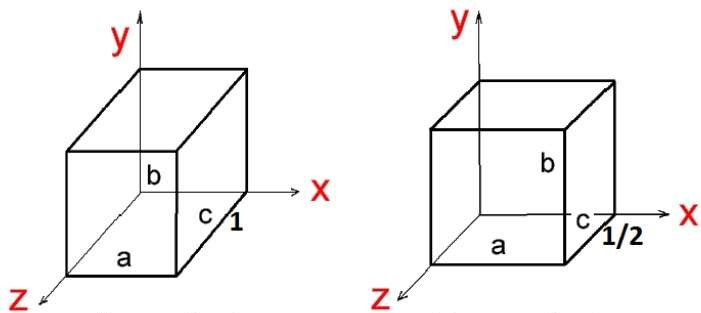
\includegraphics[width=0.6\textwidth]{images/Cavalier-Cabinet.jpg}
\caption{Προβολή \textlatin{Cavalier} (αριστερά) και προβολή \textlatin{Cabinet} (δεξιά)}
\end{figure}

Τη θεωρητική εξέταση του αντικειμένου της εργασίας θα ακολουθήσει η υλοποίηση ενός απλού προγράμματος στην προγραμματιστική γλώσσα \textlatin{C++} με τη χρήση του λογισμικού \textlatin{OpenGL}, το οποίο θα επιτρέπει στον χρήστη τη διαδραστική περιστροφή του μοναδιαίου κύβου πέριξ των αξόνων $x$, $y$ ή $z$. Αναγκαία είναι η δημιουργία τριών παραθύρων για την απεικόνιση μιας προοπτικής προβολής, της πλάγιας προβολής \textlatin{Cavalier} και της πλάγιας προβολής \textlatin{Cabinet} αντιστοίχως. \par

\chapter{Θεωρητικό υπόβαθρο}

Σε μια σκήνη τριών διαστάσεων, κάθε αντικείμενο ορίζεται από ένα σύνολο επιφανειών, σχηματίζοντας ένα κλειστό σύνολο γύρω από το εσωτερικό του αντικειμένου. Ωστόσο, υπάρχει ανάγκη για προβολή των εσωτερικών στοιχείων ή όψεων των τομών ενός αντικειμένου και για επεξεργασία της περιγραφής των αντικειμένων, προβάλλοντας μια καθορισμένη όψη τους πάνω στην επιφάνεια μιας συσκευής παρουσίασης. Συνεπώς, συγκριτικά με τη διδιάστατη απεικόνιση, η μεταφορά της σκηνής σε μια προβολή πάνω σε μια επίπεδη επιφάνεια απαιτεί τον εντοπισμό των ορατών τμημάτων μιας σκηνής, καθώς και τον υπολογισμό των εφέ φωτισμού και των χαρακτηριστικών των επιφανειών. \par

Η λήψη μιας προβολής 3Δ σκηνής παγκοσμίων συντεταγμένων απαιτεί και τον ορισμό αναφοράς συντεταγμένων θέασης. Αυτή ορίζει τη θέση και τον προσανατολισμό ενός επιπέδου θέασης, το οποίο αντιστοιχεί στο επίπεδο ενός φανταστικού φιλμ μιας κάμερας. Στη συνέχεια, οι περίγραφες των αντικειμένων μεταφέρονται στις συντεταγμένες αναφοράς θέασης σε μορφή περιγράμματος ή με την εφαρμογή τεχνικών φωτισμού και απόδοσης. Γενικώς, κατά τον μετασχηματισμό προβολής δεν διατηρούνται οι αναλογίες των αποστάσεων (\textlatin{Hearn \& Baker}, 2010, σ. 331). \par

Όσον αφορά την προβολή, αυτή δύναται να οριστεί ως η δημιουργία της εικόνας ενός αντικειμένου πάνω σε ένα απλούστερο αντικείμενο\footnote{Το απλούστέρο αντικείμενο προβολής είναι το επίπεδο ή μια επιφάνεια.}. Οι ευθείες προβολών ορίζονται από το κέντρο προβολής και τα προβαλλόμενα σημεία. Σε μια 3Δ σκηνή δύνανται να επιλεχθούν διαφορετικές μέθοδοι προβολής της σκηνής πάνω στο επίπεδο θέασης. Τα είδη των προβολών χωρίζονται σε παράλληλες προβολές (\textlatin{parallel projections}) και προοπτικές προβολές (\textlatin{perspective projections}). Ειδικώς, παράλληλη ονομάζεται η προβολή κατά την οποία τα σημεία της επιφάνειας του αντικειμένου προβάλλονται κατά μήκος παραλλήλων γραμμών και κύριο χαρακτηριστικό της είναι η ακριβής προβολή των διαστάσεων του προβαλλόμενου αντικειμένου, ενώ προοπτική ονομάζεται η προβολή κατά την οποία τα σημεία της επιφάνειας ενός αντικειμένου προβάλλονται κατά μήκος ιχνών που συγκλίνουν. Κύριο χαρακτηριστικό της τελευταίας είναι η ρεαλιστικότατά της (Μουστάκας κ.ά., 2015? \textlatin{Hearn \& Baker}, 2010). \par

Περεταίρω διαχωρισμός των δύο βασικών κατηγοριών προβολών δύναται να είναι ο απεικονιζόμενος εις την ακόλουθη εικόνα. \par

\begin{figure}[h]
\centering
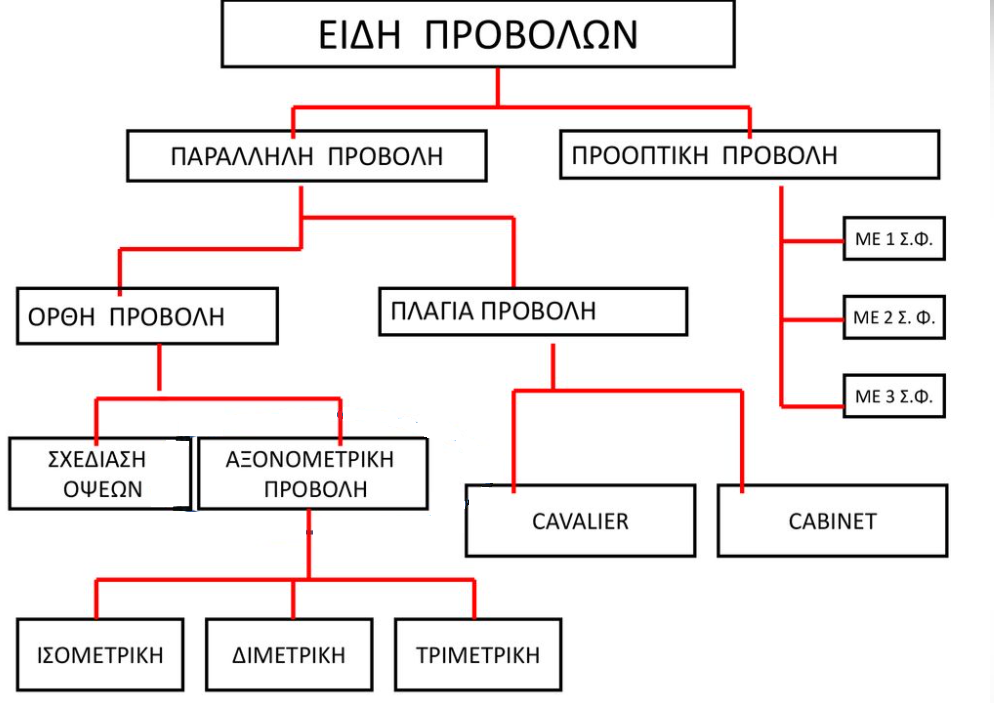
\includegraphics[width=0.75\textwidth]{images/projection}
\caption{Είδη προβολών}
\end{figure}

\hspace{0.5em}

Παρατηρώντας το παραπάνω σχήμα, διαπιστώνεται πως οι πλάγιες προβολές, το αντικείμενο ανάλυσης της παρούσας εργασίας, είναι υποκατηγορία των παραλλήλων προβολών. Γενικώς, πλάγια παράλληλη προβολή ονομάζεται η χαρτογράφηση κατά την οποία το ίχνος προβολής δεν είναι κάθετο στο επίπεδο θέασης. Οι πλάγιες προβολές ορίζονται από τη διεύθυνση ενός διανύσματος για τις γραμμές προβολής. \par

Δύο σημαντικές περιπτώσεις πλάγιας προβολής σε σχεδιαστικές εφαρμογές, όπως βλέπουμε και στην Eικόνα 1.1, αποτελούν οι \textlatin{Cavalier} με γωνία ύψους $45\degree$ και \textlatin{Cabinet} με γωνία ύψους $63\degree$. Προβολές \textlatin{Cavalier} ονομάζονται οι όψεις που λαμβάνουμε όταν η γωνία $a = 45\degree$ με $\tan a = 1$, όπου όλες οι γραμμές κάθετες του επιπέδου προβολής προβάλλονται χωρίς αλλαγή στο μήκος, ενώ προβολές \textlatin{Cabinet} χαρακτηρίζονται οι όψεις λαμβανόμενες για γωνία  $a = 63\degree$ με $\tan a = 2$. Σε αυτή την περίπτωση, οι γραμμές παράλληλες στην επιφάνεια θέασης προβάλλονται στο μισό του μήκους τους με αποτέλεσμα να φαίνονται πιο ρεαλιστικές εξαιτίας της μείωσης των καθέτων. \par

Στην ακόλουθη εικόνα απεικονίζεται παράδειγμα προβολής \textlatin{Cavalier} κύβου πάνω σε ένα επίπεδο θέασης για δύο τιμές της γωνίας $φ$, όπου το βάθος του κύβου προβάλλεται με μήκος ίσο με αυτό του πλάτους και του ύψους, καθώς και παράδειγμα προβολής \textlatin{Cabinet} κύβου πάνω σε ένα επίπεδο θέασης για δύο τιμές της γωνίας $φ$, όπου το βάθος προβάλλεται με μήκος μισό του πλάτους και του ύψους του κύβου (Σπύρου, 2019? \textlatin{Hearn \& Baker}, 2010). \par

\begin{figure}[h]
\centering
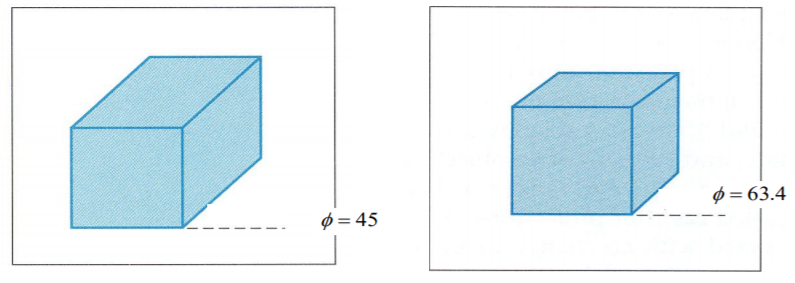
\includegraphics[width=0.75\textwidth]{images/projectionCabinet-Cavalier}
\caption{Παράδειγμα πλαγίων προβολών \textlatin{Cavalier}-\textlatin{Cabinet} }
\end{figure}
\chapter{Υπόδειξη μέτρησης μηκών ακμών σε προβολή \textlatin{Cavalier} και \textlatin{Cabinet}}

\counterwithout{equation}{chapter} % αφαιρεί αριθμό κεφαλαίου από τον αριθμό κάθε εξίσωσης

Στην ενότητα αυτή θα υλοποιηθεί η μέτρηση μηκών των προβολών των ακμών μοναδιαίου κύβου, οι οποίες αρχικώς ήταν κάθετες, και θα βρεθούν οι πλάγιες προβολές \textlatin{Cavalier} και \textlatin{Cabinet} του κύβου αυτού στο επίπεδο $x-y$ με τη χρήση γωνίας αζιμουθίου ίση με $60\degree$. Ως οδηγός για την επίλυση του προαναφερθέντος ζητήματος επιλέγεται παράδειγμα που προσδιορίζει το μητρώο πλαγίων προβολών καθορισμένων με γωνίες αζιμουθίου και ανύψωσης $φ$ και $θ$ αντιστοίχως, οι οποίες ορίζουν τη σχέση της κατεύθυνσης προβολής προς το επίπεδο προβολής (Δρακόπουλος, 2022).

\section{Πλάγια προβολή \textlatin{Cavalier}}
Αρχικώς, μελετούμε την πλάγια προβολή \textlatin{Cavalier}. Σε αυτή, απαιτείται γωνία ανύψωσης $θ = 45\degree$ και γωνία της επιλογής μας $φ = 60\degree$. Συγκεκριμένα, υποθέτουμε πως έχουμε μοναδιαίο κύβο με τον ακόλουθο πίνακα κορυφών.

\vspace{0.5em}

\begin{equation}
\textlatin{C} = \left(\begin{array}{rrrrrrrrr}
0 & 1 & 1 & 0 & 0 & 0 & 1 & 1\\
0 & 0 & 1 & 1 & 1 & 0 & 0 & 1\\
0 & 0 & 0 & 0 & 1 & 1 & 1 & 1\\
1 & 1 & 1 & 1 & 1 & 1 & 1 & 1\\
\end{array}\right)
\end{equation}\\
\\
Επίσης, υποθέτουμε πως $x-y$ είναι το επίπεδο στο οποίο προβάλλεται ο προαναφερθής μοναδιαίος κύβος. Το διάνυσμα κατεύθυνσης της προβολής είναι:\\
\begin{equation}
\overrightarrow{\textlatin{DOP}} = \left(\begin{array}{rrr}
\cos\theta \cos\phi, \cos\theta \sin\phi, \sin\theta
\end{array}\right)^{\mathrm T}
\end{equation}\\
όπου $φ$ είναι ο αριθμός αζιμουθίου και $θ$ η ανύψωση. Με αντικατάσταση των συνημιτόνων των γωνιών $φ$ και εφαπτομένων της γωνίας των  $60\degree$ και $θ$ της γωνίας ανύψωσης για την πλάγια προβολή \textlatin{Cavalier} στον παρακάτω πίνακα\\
\begin{equation}
\textlatin{Ρoblique}(\phi, \theta) = \left(\begin{array}{rrrr}
1 & 0 & -\cos\theta/\tan\theta & 0\\
0 & 1 & -\sin\phi/\tan\phi  & 1 \\
0 & 0 &     0 & 0 \\
0 & 0 &     0 & 1 \\
\end{array}\right)
\end{equation} \\
προκύπτει ο εξής πίνακας:\\
\begin{equation}
\textlatin{Ρoblique} (60, 45) = \left(\begin{array}{rrrr}
1 & 0 & -\surd2/2 & 0\\
0 & 1 & -1/2  & 1 \\
0 & 0 &  0 & 0 \\
0 & 0 & 0 & 1 \\
\end{array}\right)
\end{equation} \\

Στη συνέχεια, πραγματοποιείται πολλαπλασιασμός μεταξύ του \textlatin{POBLIQUE} και του πίνακα $C$ του μοναδιαίου κύβου και προκύπτει ο παράγων πίνακας. Ακολούθως, παρατηρούμε ποιες προβολές υπήρξαν κάθετες στο επίπεδο $x-y$ και λαμβάνουμε νόρμα μεταξύ των σημείων που ενώνονται σε κάθε προβολή. Εξετάζοντας τα αποτελέσματα των παραπάνω πράξεων, συμπεραίνουμε πως στις πλάγιες προβολές \textlatin{Cavalier} το αποτέλεσμα της νόρμας των δύο σημείων που ενώνονται σε κάθε προβολή είναι ίδιο με τον αρχικό αριθμό μήκους.

\section{Πλάγια προβολή \textlatin{Cabinet}}

Σε αυτό το σημείο, μελετάται η επίλυση της πλάγιας προβολής \textlatin{Cabinet}. Η προβολή \textlatin{Cabinet} απαιτεί γωνία ανύψωσης $θ = 63\degree$  και γωνία της επιλογής μας $φ = 60\degree$. Συγκεκριμένα, υποθέτουμε πως έχουμε τον ίδιο μοναδιαίο κύβο και το ίδιο επίπεδο προβολής $x-y$ με την προηγούμενη υλοποίηση. Το διάνυσμα κατεύθυνσης της προβολής και σε αυτή την περίπτωση είναι:\\
\begin{equation}
\overrightarrow{\textlatin{DOP}} = \left(\begin{array}{rrr}
\cos\theta\cos\phi, \cos\theta\sin\phi, \sin\theta
\end{array}\right)^{\mathrm T}
\end{equation} \\
όπου $φ$ είναι ο αριθμός αζιμουθίου και $θ$ η ανύψωση. Με αντικατάσταση των συνημίτονων των γωνιών $φ$ και εφαπτομένων της γωνίας των $60\degree$ και $θ$ της γωνίας ανύψωσης για την πλάγια προβολή \textlatin{Cabinet} στον παρακάτω πίνακα\\
\begin{equation}
\textlatin{Ρoblique}(\phi, \theta) = \left(\begin{array}{rrrr}
1 & 0 & -\cos\theta/\tan\theta & 0\\
0 & 1 & -\sin\phi/\tan\phi  & 1 \\
0 & 0 &     0 & 0 \\
0 & 0 &     0 & 1 \\
\end{array}\right)
\end{equation} \\
προκύπτει ο εξής πίνακας:\\
\begin{equation}
\textlatin{Ρoblique}(60, 63) = \left(\begin{array}{rrrr}
1 & 0 & -5 & 0\\
0 & 1 & -1/2  & 1 \\
0 & 0 &  0 & 0 \\
0 & 0 & 0 & 1 \\
\end{array}\right)
\end{equation} \\

Στη συνέχεια, πραγματοποιείται πολλαπλασιασμός μεταξύ του \textlatin{POBLIQUE} και του πίνακα $C$ του μοναδιαίου κύβου και προκύπτει ο παράγων πίνακας. Ακολούθως, παρατηρούμε ποιες προβολές υπήρξαν κάθετες στο επίπεδο $x-y$ και λαμβάνουμε νόρμα μεταξύ των σημείων που ενώνονται σε κάθε προβολή. Εξετάζοντας τα αποτελέσματα των παραπάνω πράξεων, συμπεραίνουμε πως στις πλάγιες προβολές \textlatin{Cabinet} το αποτέλεσμα της νόρμας των δύο σημείων που ενώνονται σε κάθε προβολή είναι μισό του αρχικού μήκους (Δρακόπουλος, 2022). \par

\chapter{Υλοποίηση κώδικα}

Το βασικότερο μέλημα της παρούσας εργασίας είναι η δημιουργία ενός προγράμματος (\textattachfile[color = 0 0 1]{program.cpp}{\textlatin{program.cpp}}) διαδραστικής περιστροφής μοναδιαίου κύβου πέριξ των αξόνων $x$, $y$ και $z$, καθώς και η απεικόνιση των προβολών προοπτικής, \textlatin{Cavalier} και \textlatin{Cabinet} του κύβου αυτού. Το πρόγραμμα έχει δημιουργηθεί σε κώδικα \textlatin{C++}, με τη χρήση του λογισμικού \textlatin{OpenGL}. Για την ανάπτυξη του κώδικα συμβουλευτήκαμε τους Δρακόπουλο (2022), Γκάνια (2016) και \textlatin{Thormählen} (2021). Ακολουθεί η εξήγηση του προγράμματος, το οποίο δύναται να χωριστεί σε έξι βασικά στάδια. \par

Αρχικό βήμα της υλοποίησης είναι η δήλωση των απαραίτητων βιβλιοθηκών, τόσο αυτών της \textlatin{OpenGL} όσο και μαθηματικών συναρτήσεων και αλφαριθμητικών, καθώς και η δήλωση των διαστάσεων του παραθύρου. Στο δεύτερο στάδιο δηλώνουμε τους τρεις τύπους απεικονιζόμενων προβολών - ισομετρική προβολή, προβολή \textlatin{Cavalier} και προβολή \textlatin{Cabinet} - θέτοντας την ισομετρική ως την προκαθορισμένη προβολή εμφανιζόμενη κατά τη δημιουργία παραθύρου απεικόνισης. Στη συνέχεια, σχεδιάζουμε τον μοναδιαίο κύβο με τη χρήση της εντολής \textlatin{GL\_LINE\_LOOP} της \textlatin{OpenGL}, καθώς και τους άξονες $z$, $x$ και $y$ με τη χρήση της εντολής \textlatin{GL\_LINES}. Ο σχεδιασμός των δύο τελευταίων βασίζεται στη διαδικασία δημιουργίας του πρώτου άξονα και του βέλους κατεύθυνσής του, το οποίο σχεδιάζεται με τις εντολές \textlatin{GL\_TRIANGLES} και \textlatin{GL\_POLYGON}. \par

Το τρίτο στάδιο αποτελείται από τη συνάρτηση απεικόνισης \emph{\textlatin{handleRender()}}. Η συνάρτηση αυτή ορίζει το μητρώο ταυτότητας (\textlatin{identity matrix}), υπολογίζοντας τις γωνίες και τα μητρώα της ισομετρικής προβολής και των πλάγιων προβολών \textlatin{Cavalier} και \textlatin{Cabinet}. Επιπροσθέτως, σχεδιάζει τους τρεις άξονες, καλώντας τις αντίστοιχες συναρτήσεις και χρωματίζοντας μπλε τον άξονα $z$, πράσινο τον άξονα $y$ και κόκκινο τον άξονα $x$. Τέλος, καλεί τη συνάρτηση σχεδιασμού του μοναδιαίου κύβου. \par

Κατά το τέταρτο βήμα, ορίζουμε τη συνάρτηση ανακαθορισμού μεγέθους του παραθύρου \emph{\textlatin{handleReshape()}}, η οποία ορίζει το επίπεδο και τα $x$, $y$, $w$, $h$ με την χρήση των εντολών \textlatin{glViewport} και \textlatin{glOrtho}. Αναλυτικότερα, τα $x$ και $y$ καθορίζουν την κάτω αριστερά γωνία της θύρας προβολής σε \textlatin{pixel}, ενώ το πλάτος $w$ και το ύψος $h$ αντιπροσωπεύουν το ορθογώνιο προβολής, σχεδιάζοντας ξανά το παράθυρο σύμφωνα με τις αλλαγές. Έπειτα ακολουθεί το πέμπτο στάδιο, δηλαδή η συνάρτηση αλληλεπίδρασης με το πληκτρολόγιο \emph{\textlatin{handleKeydown()}}. Η συνάρτηση αυτή επιτρέπει στον χρήστη να επιλέξει την επιθυμητή προβολή προς απεικόνιση, αντιστοιχίζοντας το πλήκτρο "1" στην ισομετρική προβολή, το πλήκτρο "2" στην προβολή \textlatin{Cavalier} και το πλήκτρο "3" στην προβολή \textlatin{Cabinet}. \par

Στο τελευταίο στάδιο δομείται η βασική συνάρτηση του προγράμματος, δηλαδή η \emph{\textlatin{main}} συνάρτηση, κατά την οποία ορίζεται ο τύπος και το παράθυρο απεικόνισης, δημιουργείται το προαναφερθέν παράθυρο και καλούνται οι συναρτήσεις απεικόνισης, ανασχηματισμού και επικοινωνίας με το πληκτρολόγιο, ώστε να εμφανιστεί στην οθόνη του χρήστη το παράθυρο των προβολών.

\newpage
% Συμπεράσματα

\addcontentsline{toc}{chapter}{Συμπεράσματα}
\chapter*{Συμπεράσματα}

Όπως έχει ήδη αναφερθεί, σκοπός της παρούσας εργασίας ήταν ο υπολογισμός των μηκών των πλαγίων προβολών \textlatin{Cavalier} και \textlatin{Cabinet} ενός μοναδιαίου κύβου στο επίπεδο $x-y$ με τη χρήση γωνίας αζιμουθίου, η υλοποίηση προγράμματος διαδραστικής περιστροφής του μοναδιαίου κύβου πέριξ των αξόνων $x$, $y$ και $z$, και η απεικόνιση των πλαγίων προβολών \textlatin{Cavalier} και \textlatin{Cabinet} και της προοπτικής προβολής σε τρία διαφορετικά παράθυρα. Όπως διαπιστώθηκε, ο υπολογισμός των μηκών των ακμών του κύβου, έχοντας εφαρμόσει πλάγια προβολή \textlatin{Cavalier} και \textlatin{Cabinet}, είναι εφικτός και δύναται να υλοποιηθεί με τον τρόπο που υποδείχθηκε στη θεωρητική υλοποίηση. Ως προς το δεύτερο ζητούμενο της εργασίας, συμπεράναμε πως η υλοποίηση στο λογισμικό \textlatin{OpenGL} ήταν εφικτή αλλά όχι και τόσο αβίαστη. \par

Δοθέντος αρκετού χρόνου για εμβάθυνση στο θέμα της εργασίας και εξοικείωση με την προαναφερθείσα προγραμματιστική πλατφόρμα, στοχεύουμε στην εξέταση και βελτιστοποίηση της υλοποίησης διαδραστικής περιστροφής μονοδιαίου κύβου και δημιουργίας πολλαπλών παραθύρων. Στους μελλοντικούς μας στόχους συμπεριλαμβάνεται και η μελέτη των υπολοίπων κατηγοριών προβολών αναφερθόντων επιγραμματικώς στο πλαίσιο της παρούσας εργασίας.

% Επίλογος

\addcontentsline{toc}{chapter}{Επίλογος}
\chapter*{Επίλογος}

Εν κατακλείδι, ο υπολογισμός των μηκών των ακμών κύβου των πλαγίων προβολών \textlatin{Cavalier} και \textlatin{Cabinet} με τη χρήση γωνίας αζιμουθίου, καθώς και η υλοποίηση του προγράμματος διαδραστικής περιστροφής κύβου και εμφάνισης τριών διαφορετικών παραθύρων προοπτικής προβολής, προβολής \textlatin{Cavalier} και προβολής \textlatin{Cabinet}, υλοποιήθηκαν με επιτυχία και έθεσαν νέους στόχους και ερωτήματα αναφορικά με τις λοιπές κατηγορίες προβολών και τους αλγορίθμους με τους οποίους αυτές επιλύονται.
\newpage
% Αναφορές

\addcontentsline{toc}{chapter}{Αναφορές}

\begin{thebibliography}{10}

% Ελληνόγλωσση βιβλιογραφία

\bibitem{1} Δρακόπουλος, Β. (2022). \emph{Εισαγωγή και Αλγόριθμοι ψηφιδόξυσης} [Πανεπιστημιακές Σημειώσεις]. Πανεπιστήμιο Θεσσαλίας, Τμήμα Πληροφορικής με Εφαρμογές στη Βιοϊατρική, Π.Π.Σ.: "Γραφική Υπολογιστών", Εαρινό Εξάμηνο 2020-2021, Λαμία.

\bibitem{2} Μουστάκας, Κ., Παλιόκας, Ι., Τζοβάρας, Δ., \& Τσακίρης, Α. (2015). \textit{Γραφικά και Εικονική Πραγματικότητα} [ηλεκτρ. βιβλ.]. Αθήνα: Σύνδεσμος Ελληνικών Ακαδημαϊκών Βιβλιοθηκών. \textlatin{\url{http://hdl.handle.net/11419/4491}}

\bibitem{3} Σπύρου, Ε. (2018-2019). \textit{4ο Μάθημα – Προβολές και Μετασχηματισμοί} [Πανεπιστημιακές Σημειώσεις]. Πανεπιστήμιο Θεσσαλίας, Τμήμα Πληροφορικής και Τηλεπικοινωνιών, Π.Π.Σ.: "Γραφικά", Εαρινό Εξάμηνο 2018-2019, Λαμία. 
\textlatin{\url{http://archive.eclass.uth.gr/eclass/modules/document/file.php/INFS206/grafika-04.pdf}}

\bibitem{4} \textlatin{Hearn, D., \& Baker, M. P.} (2010). \emph{Γραφικά Υπολογιστών με \textlatin{OpenGL}} (Π. Μποζάνης, Επιμ.) (Γ. Σίσιας, Μετάφ.) (3η έκδ.). Θεσσαλονίκη: ΤΖΙΟΛΑ. (Το πρωτότυπο έργο δημοσιεύτηκε το 1986).

\bibitem{5} Γκάνιας, Α. (2016). \textit{Γραφικά Υπολογιστών} [Πτυχιακή Εργασία]. Ιδρυματικό αποθετήριο πρώην ΤΕΙ Ηπείρου. \textlatin{\url{https://apothetirio.lib.uoi.gr/xmlui/bitstream/handle/123456789/5432/1425.pdf?sequence=1}}


% Ξενόγλωσση βιβλιογραφία

\bibitem{6} \textlatin{Thormählen, T. (2021). \emph{Graphics Programming Cameras: Parallel Projection}. Phillips, Universitat Marburg}. Ανακτήθηκε από: \textlatin{\url{www.mathematik.uni-marburg.de/~thormae/lectures/graphics1/graphics_6_2_eng_web.html?fbclid=IwAR1FpJMp7yNVS2AYS4LQyL7M_KRFkWKv933Wv1KLF-V9A9JC1dVKBb6twT0#1}}

\end{thebibliography}


\end{document}
